%==============================================================================
%  SuperMoTo — 2.1 Monitor + Subwoofer Quickstart Guide
%
%  Build:  pdflatex quickstart.tex   (run twice for cross-references)
%
%  (c) 2023-2026 Olivier Doaré — LGPL-3.0-or-later
%==============================================================================
\documentclass[11pt,a4paper]{article}

\usepackage[utf8]{inputenc}
\usepackage[T1]{fontenc}
\usepackage{lmodern}
\usepackage[margin=2.5cm]{geometry}
\usepackage{graphicx}
\usepackage{xcolor}
\usepackage{tikz}
\usetikzlibrary{positioning,arrows.meta,calc,fit,backgrounds,shapes.geometric}
\usepackage{pgfplots}
\pgfplotsset{compat=1.17}
\usepackage{booktabs}
\usepackage{tabularx}
\usepackage{enumitem}
\usepackage{amsmath}
\usepackage{amssymb}
\usepackage{siunitx}
\usepackage{fancyhdr}
\usepackage[colorlinks=true,linkcolor=smtblue,urlcolor=smtblue,citecolor=smtblue]{hyperref}

%-- Theme colours (matching Theme.h & SuperMoTo manual) -----------------------
\definecolor{smtblue}{HTML}{2E6DB4}
\definecolor{smtgold}{HTML}{C9A227}
\definecolor{smtpanel}{HTML}{2B2F36}
\definecolor{smtlight}{HTML}{EEF1F5}
\definecolor{smtgreen}{HTML}{3FA34D}
\definecolor{smtred}{HTML}{B4472E}
\definecolor{smtgls}{HTML}{6E5A85}

%-- Screenshot placeholder command ---------------------------------------------
\newcommand{\screenshot}[2]{%
  \begin{figure}[ht]
  \centering
  \IfFileExists{figures/quickstart/#1}{%
    \includegraphics[width=0.88\textwidth]{figures/quickstart/#1}%
  }{%
    \fbox{\parbox[c][0.20\textwidth][c]{0.86\textwidth}{\centering
      \itshape [Screenshot Suggestion: \texttt{#1}]\par\medskip
      \normalfont\footnotesize #2}}%
  }%
  \caption{#2}
  \label{fig:#1}
  \end{figure}}

\pagestyle{fancy}
\fancyhf{}
\setlength{\headheight}{14pt}
\rhead{\textsc{SuperMoTo} — Quickstart Guide: 2.1 Setup}
\lhead{\leftmark}
\rfoot{\thepage}

\title{{\Huge\textbf{SuperMoTo Quickstart Guide}}\\[0.4em]
       \Large Step-by-Step Setup: Stereo Monitors + Subwoofer (2.1 Configuration)\\[0.8em]
       \large Calibration, Subwoofer Alignment, FIR Correction \& System Verification}
\author{Olivier Doaré, ENSTA / FX-Mechanics\\
\href{https://github.com/odoare/SuperMoTo}{\texttt{github.com/odoare/SuperMoTo}}}
\date{\today \quad|\quad Document version 1.0}

\begin{document}
\maketitle

\begin{abstract}
\noindent This quickstart guide provides a comprehensive, step-by-step walkthrough for setting up, measuring, time-aligning, correcting, and verifying a standard 2.1 monitoring system (a pair of stereo studio monitors plus an active subwoofer) using \textbf{SuperMoTo}. Following this workflow ensures optimal crossover phase alignment, seamless low-end integration, and accurate room correction across the listening seat.
\end{abstract}

\tableofcontents
\vspace{0.8cm}
\hrule
\vspace{0.8cm}

%==============================================================================
\section{System Topology \& Calibration Workflow}
%==============================================================================

Integrating a subwoofer with stereo main monitors involves two distinct challenges:
\begin{enumerate}[nosep]
  \item \textbf{Magnitude response shaping:} Equalising room modes, speaker-boundary interference (SBIR), and tonal imbalance for each driver.
  \item \textbf{Crossover phase alignment:} Ensuring the mains and subwoofer add constructively (in phase) through the crossover region (typically \SI{80}{\hertz}), avoiding deep cancellation dips.
\end{enumerate}

\noindent \textbf{SuperMoTo} separates routing/crossover management from physical loudspeaker correction. Routing and crossovers live on matrix \emph{configurations} (A--F), while speaker-specific FIR filters, gain trims, delays, and polarities live directly on physical \emph{outputs} (Section~\ref{sec:step1}).

\paragraph{Recommended DAW Insertion:}
The best and recommended way to use SuperMoTo is to insert the plugin into the dedicated \textbf{monitoring section} of your DAW. This workflow has been fully tested in \textbf{Cockos REAPER} using its \textit{Monitoring FX} chain, where the plugin operates globally across project loads without affecting offline project rendering or master mix buses. Refer to Chapter~2 (\textit{DAW Hosts \& Setup}) of the full SuperMoTo manual (\texttt{SuperMoTo.tex}) for host-specific details and routing guidelines across different DAWs.

\begin{table}[ht]\centering
\begin{tabularx}{\textwidth}{l l X}
\toprule
\textbf{Channel} & \textbf{Physical Assignment} & \textbf{Role} \\
\midrule
Input 1 & DAW Master Left & Stereo source feed (Left) \\
Input 2 & DAW Master Right & Stereo source feed (Right) \\
Output 1 & Left Main Monitor & High-passed main speaker + FIR correction + Delay \\
Output 2 & Right Main Monitor & High-passed main speaker + FIR correction + Delay \\
Output 3 & Active Subwoofer & Low-passed subwoofer + Bulk delay + Polarity \\
\bottomrule
\end{tabularx}
\caption{Standard channel mapping for a 2.1 monitoring setup.}\label{tab:channel-map}
\end{table}

%-- Diagram of the signal flow ------------------------------------------------
\begin{figure}[ht]
\centering
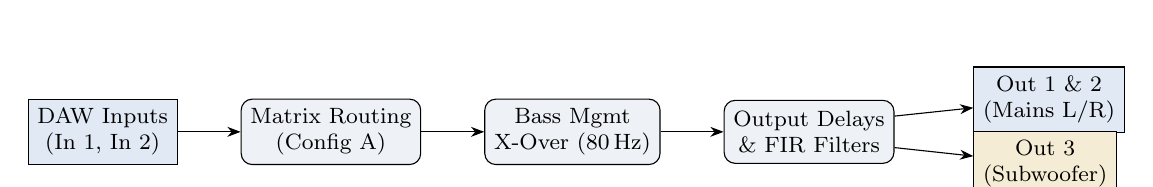
\begin{tikzpicture}[
   node distance=5mm and 8mm,
   block/.style={draw, rounded corners, fill=smtlight, minimum height=8mm,
                 minimum width=18mm, align=center, font=\footnotesize},
   io/.style={draw, fill=smtblue!15, minimum height=8mm, minimum width=15mm,
              align=center, font=\footnotesize},
   sub/.style={draw, fill=smtgold!20, minimum height=8mm, minimum width=18mm,
              align=center, font=\footnotesize},
   >={Stealth[]}]
  \node[io] (in) {DAW Inputs\\(In 1, In 2)};
  \node[block, right=of in] (matrix) {Matrix Routing\\(Config A)};
  \node[block, right=of matrix] (xover) {Bass Mgmt\\X-Over (\SI{80}{\Hz})};
  \node[block, right=of xover] (proc) {Output Delays\\\& FIR Filters};
  \node[io, right=10mm of proc.north east, anchor=west] (mains) {Out 1 \& 2\\(Mains L/R)};
  \node[sub, right=10mm of proc.south east, anchor=west] (sub) {Out 3\\(Subwoofer)};
  
  \draw[->] (in) -- (matrix);
  \draw[->] (matrix) -- (xover);
  \draw[->] (xover) -- (proc);
  \draw[->] ($(proc.east)+(0,2mm)$) -- (mains);
  \draw[->] ($(proc.east)-(0,2mm)$) -- (sub);
\end{tikzpicture}
\caption{Signal flow of the 2.1 setup in SuperMoTo: stereo inputs are routed through configuration matrix A, filtered by the \SI{80}{\hertz} crossover, processed by output FIRs and delays, and delivered to the mains and subwoofer.}
\label{fig:signal-flow}
\end{figure}

%-- Overview of the 5-step loop -----------------------------------------------
\begin{table}[ht]\centering
\begin{tabularx}{\textwidth}{c l l X}
\toprule
Step & Phase & Mode / Tool & Objective \\
\midrule
1 & Configuration & Config Tool & Apply 2.1 layout: \SI{80}{\hertz} crossover, bass management to Config~A \\
2 & Measurement & Calibration ("Dry") & Capture raw acoustic sweeps for Out 1, Out 2, and Sub (Out 3) \\
3 & Alignment \& FIR & Group Analysis & Calculate delays, sub phase alignment, and export FIR filters \\
4 & Verification & Calibration ("System") & Re-measure DAW inputs to validate flat response and crossover sum \\
5 & Target Curve & Target View & Select and engage downward tilt (e.g., Moderate \SI{-4}{\dB}) \\
\bottomrule
\end{tabularx}
\caption{The five-step setup loop for a 2.1 monitoring system.}\label{tab:workflow-loop}
\end{table}

\screenshot{welcome.png}{SuperMoTo after loading, with a 2x8 empty matrix.}

\clearpage

%==============================================================================
\section{Step 1: Routing \& Bass Management Setup}\label{sec:step1}
%==============================================================================

Before taking measurements, configure the plugin matrix so that low-frequency content from both stereo channels is routed to the subwoofer, while the main monitors receive high-passed audio.

\begin{enumerate}
  \item Insert \textbf{SuperMoTo} onto your DAW's Monitoring FX chain (e.g., in REAPER) or Master Track. Ensure the plugin has at least 2 inputs and 3 outputs active.
  \item Open the \textbf{Configuration tool} pane (or click the Config button on the main toolbar).
  \item Configure the settings as follows:
    \begin{itemize}[nosep]
      \item \textbf{Preset Layout:} Select \textbf{Stereo 2.1}.
      \item \textbf{Left channel:} Assign to \textbf{Output 1}.
      \item \textbf{Right channel:} Assign to \textbf{Output 2}.
      \item \textbf{Subwoofer channel:} Assign to \textbf{Output 3}.
      \item \textbf{Crossover frequency:} Set to \textbf{\SI{80}{\hertz}} (standard 4th-order Linkwitz-Riley crossover alignment).
      \item \textbf{Bass Management:} Keep checked (\textbf{ON}).
      \item \textbf{Write to config:} Select \textbf{Config A}.
    \end{itemize}
  \item Click \textbf{Apply to configuration}.
\end{enumerate}

\screenshot{config.png}{The Configuration tool setup for a Stereo 2.1 system. Setting the crossover to \SI{80}{\hertz} with Bass Management enabled writes highpass filters on Outputs 1-2, a lowpass filter on Output 3, and routes the sum of Inputs 1-2 to Output 3.}

\paragraph{What SuperMoTo generates:}
\begin{itemize}[nosep]
  \item Active matrix frame \texttt{In1 $\to$ Out1} with \SI{80}{\hertz} Highpass.
  \item Active matrix frame \texttt{In2 $\to$ Out2} with \SI{80}{\hertz} Highpass.
  \item Active matrix frames \texttt{In1 $\to$ Out3} and \texttt{In2 $\to$ Out3} feeding the Subwoofer.
  \item Subwoofer Output 3 configured with an \SI{80}{\hertz} Lowpass filter.
\end{itemize}

\paragraph{Renaming Outputs for Clarity:}
After applying the layout, you can also rename the physical outputs to something meaningful (e.g., \textit{KRK Left}, \textit{KRK Right}, \textit{Subwoofer}). Click directly on any output name strip in the matrix view to type a custom label. These custom names are shared across all configurations (A--F), displayed on the output strips, and automatically recorded in the measurement campaign manifest (\texttt{measurement.xml}).

\clearpage

%==============================================================================
\section{Step 2: Measurement Campaign (Dry Capture)}\label{sec:step2}
%==============================================================================

To design room correction filters and time-align the subwoofer, you must capture the unprocessed acoustic response ("Dry" mode) of each speaker across the listening position.

\subsection{Microphone Setup \& Calibration}
\begin{enumerate}[nosep]
  \item Connect your omnidirectional measurement microphone (e.g., UMIK-1, EMM-6, ECM8000) to an interface input.
  \item Create a new track in a fresh empty DAW project, set its input to your microphone, and arm record. This sends the microphone signal directly to \textbf{Input 1} (or whichever input channel you choose) of the SuperMoTo plugin. Mute the output of SuperMoTo to prevent feedback. The volume control is bypassed by the measurement run.
  \item Mount the microphone vertically at ear level at the listening position, pointing the capsule straight at the ceiling (\textbf{\ang{90} grazing orientation}). Pointing at the ceiling ensures that sound arriving from both Left and Right monitors hits the diaphragm at the identical \ang{90} angle.
  \item In the Calibration view, select your designated \textbf{Microphone input} (e.g., \textbf{Input 1} when using a DAW track, or \textbf{Input 3} for dedicated hardware routing).
  \item Click \textbf{Mic cal...} and load your microphone's \ang{90} calibration file (\texttt{.cal} or \texttt{.txt}).
\end{enumerate}

\screenshot{mic-cal-control.png}{Microphone input selector and Mic cal control. Loading a \ang{90} degrees calibration curve ensures microphone capsule colorations are removed prior to filter design.}

\subsection{Configuring the Dry Measurement}
In the \textbf{Calibration view}:
\begin{enumerate}[nosep]
  \item Set \textbf{Measurement Mode} to \textbf{Dry}. (This bypasses output trims, delays, and FIRs, driving the raw physical outputs directly).
  \item Set \textbf{Channel Toggles:} Tick \textbf{Output 1}, \textbf{Output 2}, and \textbf{Output 3}.
  \item Enable the \textbf{Sub} switch and set \textbf{Sub channel: 3}. (This tags Output 3 as \texttt{sub} in saved filenames).
  \item Select \textbf{Stimulus:} Logarithmic Sweep, \textbf{Duration:} \SI{10}{\second}, \textbf{Level:} \SI{-20}{\mathrm{dBFS}}.
  \item Select/Create a dedicated \textbf{Measurement Folder} (e.g., \texttt{meas\_21\_dry/}).
\end{enumerate}

\screenshot{calibration-view.png}{The Calibration view set up for a 2.1 Dry measurement campaign: Dry mode selected, Outputs 1, 2, and 3 enabled, Sub switch active on Output 3, and logarithmic sweep stimulus configured.}

\subsection{Executing Spatial Averaging}
Do not rely on a single microphone position! Narrow interference dips move with position, and correcting a single point causes harsh over-processing.
\begin{itemize}[nosep]
  \item Plan \textbf{7 to 9 positions} spread within a \SIrange{30}{50}{\cm} spatial cluster around the listening head position.
  \item Vary lateral position ($\pm\SI{20}{\cm}$), depth ($\pm\SI{15}{\cm}$), and height ($\pm\SI{10}{\cm}$).
  \item For each position, place the mic, type a brief note in \textbf{Run comment} (e.g., \texttt{pos 1 center}, \texttt{pos 2 left high}), and click \textbf{Run}.
  \item SuperMoTo automatically measures Output 1, Output 2, and Sub (Output 3) in sequence, writing \texttt{ch01\_pos00X.wav}, \texttt{ch02\_pos00X.wav}, and \texttt{sub\_pos00X.wav} to disk.
\end{itemize}

\subsection{Folder Manifests \& Automatic Updates}
Every measurement run writes its captured audio files directly into the target measurement folder, and immediately generates or updates two manifest files:
\begin{itemize}[nosep]
  \item \texttt{measurement.xml}: The machine-readable XML manifest storing measured channel outputs, speaker names, subwoofer identification, embedded microphone calibration curves, run comments, and sweep parameters. \textbf{This XML file is what Group Analysis reads first} when you click \textbf{Load measurement folder...}, allowing it to automatically populate driver counts, subwoofer channels, position numbers, and microphone calibration curves without manual file selection.
  \item \texttt{readme\_measurement.md}: A human-readable Markdown log documenting the campaign parameters, run comments, timestamps, and captured file listings for easy reference outside the plugin.
\end{itemize}

\clearpage

%==============================================================================
\section{Step 3: Analysis, Sub Alignment \& FIR Export}\label{sec:step3}
%==============================================================================

You can perform alignment and FIR correction using either \textbf{Group Analysis} (recommended, multi-speaker automated workflow) or \textbf{Single-Speaker Analysis} (detailed manual workflow).

%------------------------------------------------------------------------------
\subsection{Option A: Group Analysis Workflow (Recommended)}\label{sec:group-wf}
%------------------------------------------------------------------------------

Group analysis handles both monitors and the subwoofer in a single pass, computing exact relative delays, subwoofer phase steering, and exporting all FIR filters simultaneously.

\begin{enumerate}
  \item Open the \textbf{Group analysis} view.
  \item Click \textbf{Load measurement folder...} and select your \texttt{meas\_21\_dry/} directory.
    \begin{itemize}[nosep]
      \item SuperMoTo automatically sets \textbf{Speakers: 2}, loads Left (Out 1) and Right (Out 2), enables the \textbf{Sub} switch, and loads the Subwoofer (Out 3).
    \end{itemize}
  \item Set the shared correction parameters across the top bar:
    \begin{itemize}[nosep]
      \item \textbf{Crossover:} \textbf{\SI{80}{\hertz}}.
      \item \textbf{Smoothing:} \textbf{1/6 octave} (LF) and \textbf{1/6 octave} (HF).
      \item \textbf{Max boost:} \textbf{\SI{12}{\dB}} (prevents over-boosting narrow room nulls).
      \item \textbf{Correction level:} \textbf{1.0}.
      \item \textbf{Range:} \textbf{\SI{20}{\hertz}} to \textbf{\SI{20}{\kilo\hertz}}.
      \item \textbf{FIR length:} \textbf{4096 samples} (\SI{93}{\ms} at \SI{44.1}{\kHz}).
      \item \textbf{Phase:} \textbf{Linear phase}.
    \end{itemize}
  \item Click \textbf{Compute alignment}.
    \begin{itemize}[nosep]
      \item SuperMoTo analyzes the propagation delay of each speaker. The farthest speaker is assigned \SI{0}{\ms}, and closer speakers receive positive delays.
      \item The algorithm feeds the delay difference into the subwoofer phase alignment engine so the crossover phase is optimized.
      \item Suggested mid-band (\SIrange{500}{2000}{\hertz}) gain trims are displayed for level matching.
    \end{itemize}
  \item Check the \textbf{Invert sub} box if the sub phase alignment indicates a $180^\circ$ polarity flip yields cleaner summation across \SI{80}{\hertz}.
  \item Click \textbf{Apply \& export...}, select an output directory for the FIR files, and confirm.
\end{enumerate}

\screenshot{group-analysis-view.png}{Group Analysis view with a 2.1 setup loaded. Clicking "Compute alignment" calculates the exact inter-driver time offsets, configures subwoofer crossover phase alignment, and prepares the batch FIR export.}

\paragraph{What "Apply \& export" writes automatically:}
\begin{itemize}[nosep]
  \item Renders FIR filter files \texttt{speaker1\_correction.wav} and \texttt{speaker2\_correction.wav}.
  \item Loads FIR paths onto Output 1 and Output 2.
  \item Writes calculated bulk delays onto Output 1, Output 2, and Subwoofer Output 3.
  \item Sets Subwoofer Output 3 polarity (\textbf{Phase inv.}) if \textbf{Invert sub} was checked.
  \item Generates a complete markdown documentation report (\texttt{report.md}).
\end{itemize}

\clearpage

%==============================================================================
\section{Step 4: Matrix Inspection \& Latency Compensation}\label{sec:step4}
%==============================================================================

Open the \textbf{Matrix view} to audit the physical output settings.

\screenshot{SuperMoTo_matrix_view.png}{The Matrix view showing engaged Output strips. Outputs 1 and 2 carry their assigned FIR filters and delays. Output 3 carries the subwoofer delay and lowpass filter. The gold LED indicates active latency compensation.}

\subsection{Key Matrix Controls to Verify}
\begin{itemize}
  \item \textbf{FIR Enable \& File Paths:} Confirm Output 1 and Output 2 display green \textbf{FIR} toggles and valid wav paths.
  \item \textbf{Delays:} Confirm Output 1, Output 2, and Output 3 display their computed delay values (in \si{\ms} or samples).
  \item \textbf{Subwoofer Polarity:} Verify Output 3 has \textbf{Phase inv.} active if sub inversion was selected in the analysis.
  \item \textbf{Level Trims:} Enter any suggested level-matching trims (from Group Analysis or an SPL meter) directly into the \textbf{Trim} box of Outputs 1 and 2.
\end{itemize}

\subsection{Inter-Output Latency Compensation}
Linear-phase FIR filters introduce a processing latency equal to half the filter length ($N/2$ samples). For a 4096-sample FIR, this equals 2048 samples (\SI{46.4}{\ms} at \SI{44.1}{\kHz}).

\begin{figure}[ht]\centering

\includegraphics[width=0.45\textwidth]{figures/quickstart/latency-led.png}
\caption{The Gold Latency LED on Output strips. SuperMoTo automatically delays uncorrected or shorter-FIR outputs (such as the subwoofer on Output 3) so all active outputs remain perfectly time-aligned.}
\label{fig:latency-led}
\end{figure}

\noindent \textbf{SuperMoTo handles this automatically:} Output 3 (Subwoofer), which has no FIR filter, receives an automatic internal delay compensation so its acoustic output remains perfectly synchronized with the mains. This active alignment is indicated by a glowing \textbf{Gold LED} on the output strip (Figure~\ref{fig:latency-led}).

\clearpage

%==============================================================================
\section{Step 5: System Verification \& Validation}\label{sec:step5}
%==============================================================================

Never declare calibration complete without empirical verification! Two measurement checks validate the result.

\subsection{Check 1: Single-Speaker Correction Check ("FIR" Mode)}
\begin{enumerate}
  \item In Calibration view, select \textbf{Measurement Mode: FIR}.
  \item Measure Output 1 and Output 2 into a verification folder (e.g., \texttt{meas\_21\_fir/}).
  \item Load the captures in the Analysis view. The measured frequency response should now match the smooth predicted curve from Step 3.
\end{enumerate}

\subsection{Check 2: End-to-End System Validation ("System" Mode)}
"System" mode injects the test sweep into DAW \textbf{Inputs 1 and 2}, passing through the entire monitored path: Matrix routing, crossover filters, output delays, FIR corrections, and latency compensation.

\begin{enumerate}
  \item In Calibration view, select \textbf{Measurement Mode: System}.
  \item Select \textbf{Input 1} (Left input channel).
  \item Place the measurement microphone at the main listening position.
  \item Click \textbf{Run} to capture the complete monitored system response.
  \item Load the capture in Analysis view.
\end{enumerate}

\screenshot{validation.png}{End-to-end System validation measurement. The measured transfer function through Input 1 demonstrates a flat magnitude response and a smooth acoustic sum across the \SI{80}{\hertz} crossover without phase dips.}

\paragraph{Evaluating the Crossover Transition:}
Inspect the magnitude response around \SI{80}{\hertz}:
\begin{itemize}
  \item \textbf{Smooth, continuous sum:} Indicates correct time-alignment and phase coherence between mains and sub.
  \item \textbf{Deep dip or notch at \SI{80}{\hertz}:} Indicates phase cancellation! Toggle \textbf{Phase inv.} on Output 3 or re-check the Mains delay offset in Step 3.
\end{itemize}

\clearpage

%==============================================================================
\section{Step 6: Target Curve Selection (Target View)}\label{sec:step6}
%==============================================================================

Once your 2.1 system is corrected, time-aligned, and verified, the final setup step is selecting a \textbf{Monitor Target Curve}.

\subsection{Why a Flat In-Room Response Sounds Too Bright}
SuperMoTo's raw FIR correction aims for a flat ($0\,\mathrm{dB}$) steady-state in-room response. However, because a loudspeaker's directivity index rises with frequency and room treatment absorbs treble more than bass, a strictly flat steady-state measurement means the direct sound reaching your ears has been lifted at high frequencies. This results in an unnaturally harsh, bright monitor sound.

A gentle downward slope from bass to treble (typically $-3\,\mathrm{dB}$ to $-6\,\mathrm{dB}$ across the audio band) aligns with international monitoring standards (EBU Tech 3276, ITU-R BS.1116-3) and psychoacoustic preferences (Harman target).

\subsection{Selecting and Engaging a Target Curve}
\begin{enumerate}
  \item Open the \textbf{Target} view in SuperMoTo.
  \item Select a target curve preset from the factory bank:
    \begin{itemize}[nosep]
      \item \textbf{Flat ($0\,\mathrm{dB}$):} Raw un-tilted correction.
      \item \textbf{Gentle ($-3\,\mathrm{dB}$):} A cautious downward tilt, ideal for nearfield monitors in well-treated control rooms.
      \item \textbf{Moderate ($-4\,\mathrm{dB}$, Default):} Balanced starting point for typical control rooms.
      \item \textbf{Strong ($-6\,\mathrm{dB}$):} Steeper tilt, suitable for larger rooms or midfield listening distances.
      \item \textbf{Harman-like ($-10\,\mathrm{dB}$):} Downward tilt with a $+3\,\mathrm{dB}$ low-frequency shelf below \SI{105}{\hertz}.
      \item \textbf{Flat to \SI{1}{\kilo\hertz} ($-6\,\mathrm{dB}$):} Standard EBU Tech 3276 shape (flat below \SI{1}{\kilo\hertz}, falling over the top octaves).
    \end{itemize}
  \item Click \textbf{Engage} to activate the target curve globally across all outputs.
\end{enumerate}

\screenshot{target-curves.png}{The Target view factory target curves. Target curves apply an identical attenuation-only tilt across all active outputs, preserving main-to-subwoofer crossover phase alignment.}

\paragraph{Auditioning Reference Material:}
The target curve filter is applied identically to all outputs, ensuring the main-to-subwoofer crossover phase relationship remains completely intact. Click \textbf{Engage} on and off while auditioning familiar reference tracks to pick the tilt that produces the most natural tonal balance in your room.

\clearpage

%==============================================================================
\section{Summary Checklist \& Practical Tips}
%==============================================================================

\begin{table}[ht]\centering
\begin{tabularx}{\textwidth}{l X}
\toprule
\textbf{Task} & \textbf{Key Action / Parameter Choice} \\
\midrule
\textbf{Microphone Orientation} & Point microphone vertically at the ceiling (\ang{90}); load \ang{90} calibration file. \\
\textbf{Spatial Averaging} & Capture 7 to 9 positions within a \SIrange{30}{50}{\cm} spatial cluster around head position. \\
\textbf{Crossover Alignment} & Set \SI{80}{\hertz} in Config Tool and keep Bass Management enabled. \\
\textbf{Smoothing Baseline} & Use 1/6 octave LF and 1/6 octave HF smoothing for natural, non-spiky correction. \\
\textbf{Boost Ceiling} & Cap \textbf{Max Boost} at \SI{12}{\dB} to avoid over-driving woofers in deep acoustic nulls. \\
\textbf{Subwoofer Delays} & Allow Group Analysis to compute relative delays; do not double-count manual geometric delays. \\
\textbf{Subwoofer Polarity} & Ensure \textbf{Invert sub} in analysis matches \textbf{Phase inv.} on Output 3 in the matrix. \\
\textbf{Tracking Latency} & Use \textbf{Linear Phase} for mixing; switch to \textbf{Minimum Phase} for zero-latency tracking. \\
\textbf{Target Curve Selection} & Select Moderate (\SI{-4}{\dB}) or Gentle (\SI{-3}{\dB}) tilt in Target view and click \textbf{Engage}. \\
\bottomrule
\end{tabularx}
\caption{Quick reference checklist for 2.1 monitoring setup.}\label{tab:summary-checklist}
\end{table}

\section*{Troubleshooting \& Common Pitfalls}

\begin{description}
  \item[Symptom: Cancellation Dip at \SI{80}{\hertz}] \hfill \\
  \emph{Cause:} Subwoofer and main monitors are $180^\circ$ out of phase at the crossover frequency.\\
  \emph{Fix:} Toggle \textbf{Phase inv.} on Output 3 in the Matrix View, or re-run \textbf{Compute alignment} in Group Analysis.

  \item[Symptom: Highpass Filter Lost on Main Monitors] \hfill \\
  \emph{Cause:} Applying a layout with "Bass management" turned off removes the crossover highpass from the outputs.\\
  \emph{Fix:} Always keep "Bass management" checked when applying 2.1 layouts, or implement highpasses on matrix frames rather than outputs (Section~\ref{sec:step1}).

  \item[Symptom: Pre-Ringing or Harsh Treble] \hfill \\
  \emph{Cause:} Over-correcting sharp, non-minimum-phase room nulls due to insufficient smoothing.\\
  \emph{Fix:} Increase high-frequency smoothing (e.g., to 1/3 or 1/2 octave) and lower \textbf{Correction level} to 0.7--0.8.

  \item[Symptom: Inter-Output Delay Mismatch] \hfill \\
  \emph{Cause:} Mixing Linear-phase FIRs and Minimum-phase FIRs across active outputs.\\
  \emph{Fix:} Ensure all engaged outputs use the same phase rendering mode so latency compensation aligns all drivers consistently.
\end{description}

\end{document}
